\documentclass{article}


\usepackage{fullpage}
\usepackage{color}
\usepackage{amsmath}
\usepackage{url}
\usepackage{verbatim}
\usepackage{float}
\usepackage{graphicx}
\usepackage{parskip}
\usepackage{amssymb}
\usepackage{listings} % For displaying code
\usepackage{color} %red, green, blue, yellow, cyan, magenta, black, white
\definecolor{mygreen}{RGB}{28,172,0} % color values Red, Green, Blue
\definecolor{mylilas}{RGB}{170,55,241}
\begin{document}

\definecolor{blu}{rgb}{0,0,1}
\def\blu#1{{\color{blu}#1}}
\definecolor{gre}{rgb}{0,.5,0}
\def\gre#1{{\color{gre}#1}}
\definecolor{red}{rgb}{1,0,0}
\def\red#1{{\color{red}#1}}
\def\norm#1{\|#1\|}
\newcommand{\argmin}[1]{\mathop{\hbox{argmin}}_{#1}}
\newcommand{\argmax}[1]{\mathop{\hbox{argmax}}_{#1}}
\def\R{\mathbb{R}}
\newcommand{\fig}[2]{\includegraphics[width=#1\textwidth]{a4f/#2}}
\newcommand{\centerfig}[2]{\begin{center}\includegraphics[width=#1\textwidth]{a4f/#2}\end{center}}
\def\items#1{\begin{itemize}#1\end{itemize}}
\def\enum#1{\begin{enumerate}#1\end{enumerate}}
\def\argmax{\mathop{\rm arg\,max}}
\def\argmin{\mathop{\rm arg\,min}}
\def\half{\frac 1 2}
\newcommand{\code}[1]{\lstinputlisting[language=Matlab]{a4f/#1}}
\newcommand{\alignStar}[1]{\begin{align*}#1\end{align*}}
\newcommand{\mat}[1]{\begin{bmatrix}#1\end{bmatrix}}
\newcommand{\p}{\mathbb{P}}


\title{CPSC 540 Assignment 4 (due March 20)}
\author{Graphical Models and Paper Review}
\date{}
\maketitle
\lstset{language=Matlab,%
    %basicstyle=\color{red},
    breaklines=true,%
    morekeywords={matlab2tikz},
    keywordstyle=\color{blue},%
    morekeywords=[2]{1}, keywordstyle=[2]{\color{black}},
    identifierstyle=\color{black},%
    stringstyle=\color{mylilas},
    commentstyle=\color{mygreen},%
    showstringspaces=false,%without this there will be a symbol in the places where there is a space
    numbers=left,%
    numberstyle={\tiny \color{black}},% size of the numbers
    numbersep=9pt, % this defines how far the numbers are from the text
    emph=[1]{for,end,break},emphstyle=[1]\color{red}, %some words to emphasise
    %emph=[2]{word1,word2}, emphstyle=[2]{style},    
}

\section{Markov Chains}


\subsection{Sampling, Inference, and Decoding}

The function \emph{example\_markovChain.m} loads the initial state probabilities and transition probabilities for three Markov chain models on $d$ binary variables,
\[
p(x_1,x_2,\dots,x_d) = p(x_1)\prod_{j=2}^{d}{p(x_j|x_{j-1})}.
\]
It then tries to find the optimal decoding (the most likely assignment to the variables $\{x_1,x_2,\dots,x_d\}$) in each of the three chains. In the demo, decoding is done by enumerating all possible assignments to the variables. This works for the first two chains as they only have 4 variables, but is too slow on the last chain because it has 30 variables. In this question you'll explore two ways to estimate the marginals in third Markov chain and two ways to estimate the most-probable sequence.

\enum{
\item Write a function, \emph{sampleAncestral.m}, that uses ancestral sampling to sample sequence $x$. \blu{Hand in this code and report all the univariate marginal probabilities using a Monte Carlo estimate based on 10000 samples.}
\item Write a function, \emph{marginalCK.m}, that uses the CK equations to compute the exact univariate marginals. \blu{Hand in this code and report all exact univariate marginals.}
\item Write a function, \emph{marginalDecode.m}, that returns the sequence of states $x_j$ that maximize the marginal probability $p(x_j)$ (for each $j$). \blu{Hand in this code and report the sequence of most likely states}.
\item Write a function, \emph{viterbiDecode.m}, that implements the Viterbi decoding algorithm for Markov chains. \blu{Hand in this code and report the optimal decoding of the third Markov chain}.
}
Hint: for parts 2-4, you can use a $2$ by $d$ matrix $M$ to represent the dynamic programming table, and for part 4 you can use another matrix $B$ containing the argmax values that lead to each entry in the table. 

\subsubsection*{Solution}
\textbf{1 and 2.}
\newline
Using the script sampleAncestral.m along with the script sampleDiscrete.m to produce k samples in $\mathcal{O}(\log(k))$ we produced a $10000$ from the 
Markov Chain with 30 elements and we also calculated the exact marginals using the script marginalsCK.m. To run the scripts we used marginalsCalculation.m
shown below.
\newline
\lstinputlisting{./Question1.1/marginalCalculation.m}

The output obtained by runing the above script is the follwing
\begin{verbatim}
>>marginalCalculation

The marginals obtained using Monte Carlo estimation: 

ans =

    0.5999    0.4001
    0.4720    0.5280
    0.9035    0.0965
    0.9704    0.0296
    0.7755    0.2245
    0.2263    0.7737
    0.0533    0.9467
    0.3323    0.6677
    0.3163    0.6837
    0.6032    0.3968
    0.3505    0.6495
    0.7586    0.2414
    0.3695    0.6305
    0.1321    0.8679
    0.3646    0.6354
    0.4015    0.5985
    0.7233    0.2767
    0.7879    0.2121
    0.3122    0.6878
    0.6750    0.3250
    0.5848    0.4152
    0.2511    0.7489
    0.4032    0.5968
    0.2293    0.7707
    0.7452    0.2548
    0.6203    0.3797
    0.6039    0.3961
    0.7432    0.2568
    0.4740    0.5260
    0.4347    0.5653

The marginals obtained using CK equations: 

ans =

    0.6000    0.4000
    0.4681    0.5319
    0.8998    0.1002
    0.9718    0.0282
    0.7779    0.2221
    0.2267    0.7733
    0.0542    0.9458
    0.3359    0.6641
    0.3204    0.6796
    0.5902    0.4098
    0.3601    0.6399
    0.7479    0.2521
    0.3726    0.6274
    0.1313    0.8687
    0.3744    0.6256
    0.4103    0.5897
    0.7240    0.2760
    0.7877    0.2123
    0.3147    0.6853
    0.6698    0.3302
    0.5811    0.4189
    0.2541    0.7459
    0.4037    0.5963
    0.2403    0.7597
    0.7378    0.2622
    0.6211    0.3789
    0.6060    0.3940
    0.7419    0.2581
    0.4644    0.5356
    0.4380    0.5620
\end{verbatim}
As we can see convergence is slow, since the approximation with $10000$ samples gives accurate result to just one significant figure.
\newline

\textbf{3.}
\newline
Now we proceed to maximize the marginals, i.e. we calculate
\begin{equation*}
\max_{x_{1},\ldots,x_{30}}\p(x_{1})\ldots\p(x_{30}).
\end{equation*} 
To calculate this quatity we used the script marginalDecode.m. The output obtained shows the most likely chain given the maximization problem stated above
\begin{verbatim}
>>marginalDecode(p0,pT_long)

ans =

  Columns 1 through 13

     1     2     1     1     1     2     2     2     2     1     2     1     2

  Columns 14 through 26

     2     2     2     1     1     2     1     1     2     2     2     1     1

  Columns 27 through 30

     1     1     2     2
\end{verbatim}
The probability to obtain this chain can be easily calculated using 
\begin{equation*}
\p(1,2,1,\ldots,2,2)=\p(x_{1}=1)\p(x_{2}=2|x_{1}=1)\p(x_{3}=1|x_{1}=1)\cdots\p(x_{30}=2|x_{29}=2).
\end{equation*}
The result obtained using the probability transition matrices contained in $pT\_long(:,:,1:29)$ is
\begin{equation*}
\p(1,2,1,\ldots,2,2)=5.0639\times 10^{-5}.
\end{equation*}
In the next section we will see how this compares with the probability for the chain with highest probability.
\newline
\textbf{4.}
\newline
Now we calculate the chain with maximum probability using the script viterbiDecode.m. The results are shown below

\begin{verbatim}
>>viterbiDecode(p0,pT_long)  

ans =

  Columns 1 through 13

     1     1     1     1     1     2     2     2     2     1     2     1     2

  Columns 14 through 26

     2     2     2     2     1     2     1     1     2     2     2     1     1

  Columns 27 through 30

     1     1     1     1
\end{verbatim}
The probability to get this chain is given by
\begin{equation*}
\p(1,1,\ldots,1,1)=1.7293\times 10^{-4}.
\end{equation*}
This means that getting the chain with the maximum probability is almost 3.5 times more likely to see it than the chain that is obtained
by maximizing the marginal probabilities.


\subsection{Conditioning}

The long sequence from the previous question usually starts with state 1 and most of the time ends in state 2. In this question you'll consider conditioning on these events not happening. First, compute the following quantities which can be done using your functions from the previous question:
\enum{
\item \blu{Report all the univariate conditional probabilities $p(x_j | x_1 = 2)$ obtained using a Monte Carlo estimate based on 10000 samples}.
\item \blu{Report all the exact univariate conditionals $p(x_j | x_1 = 2)$.}
\item \blu{Report the sequence beginning with $x_1=2$ that has the highest probability.}
\item \blu{Report the sequence ending with $x_d=1$ that has the highest probability.}
}
Hint: these conditions can be done by changing the input to the functions from the previous question.

Next consider the following cases (which require implementing an extra rejection step or backward phase):
\enum{
\setcounter{enumi}{4}
\item \blu{Report all the univariate conditional probabilities $p(x_j | x_d = 1)$ obtained using a Monte Carlo estimate based on 10000 samples and rejection sampling. Also report the number of samples accepted among the 10000 samples.}
\item Write a function, \emph{sampleBackwards.m} that uses backwards sampling to sample sequences where $x_d = 1)$. \blu{Hand in this code and report all the univariate conditional probabilities $p(x_j | x_d = 1)$ obtained using a Monte Carlo estimate based on 10000 samples}.
\item Write a function, \emph{forwardBackwards.m} that is able compute all exact univariate conditionals $p(x_j | x_d = 1)$ in $O(dk^2)$. \blu{Hand in the code and report all the exact univariate conditionals $p(x_j | x_d = 1)$.}
}


\subsubsection*{Solutions}

\textbf{1 and 2}
\newline
Using the script sampleAncestral.m and using the initial probability $p0$ as $p0=[1,0]$ we produce a $10000$ samples from the Model where
every chain starts at $x_{1}=1$. With these sampeles we do a  Monte Carlo integration to approximate the marignals. Using the same
initial probability $p0$ we use the script marginalCK.m to calculate the exact conditional marginals. Below we show the results
obtained from the Monte Carlo approximation and the exact calculation of the marginals,
 where as before the $j-th$ row
in the first column is $\p(x_{j}=1|x_{1}=2)$ and the second column is $\p(x_{j}=2|x_{1}=2)$

\begin{verbatim}
>>question12
The conditional probability p(xj|x1=2) is given by: 

ans =

         0    1.0000
    0.0619    0.9381
    0.9327    0.0673
    0.9747    0.0253
    0.7754    0.2246
    0.2221    0.7779
    0.0600    0.9400
    0.3428    0.6572
    0.3142    0.6858
    0.5965    0.4035
    0.3562    0.6438
    0.7500    0.2500
    0.3777    0.6223
    0.1287    0.8713
    0.3767    0.6233
    0.4081    0.5919
    0.7273    0.2727
    0.7871    0.2129
    0.3094    0.6906
    0.6746    0.3254
    0.5877    0.4123
    0.2649    0.7351
    0.4004    0.5996
    0.2433    0.7567
    0.7336    0.2664
    0.6164    0.3836
    0.6015    0.3985
    0.7438    0.2562
    0.4595    0.5405
    0.4333    0.5667


The exact univariate conditionals are: 

M =

         0    1.0000
    0.0634    0.9366
    0.9297    0.0703
    0.9756    0.0244
    0.7789    0.2211
    0.2265    0.7735
    0.0542    0.9458
    0.3359    0.6641
    0.3204    0.6796
    0.5902    0.4098
    0.3601    0.6399
    0.7479    0.2521
    0.3726    0.6274
    0.1313    0.8687
    0.3744    0.6256
    0.4103    0.5897
    0.7240    0.2760
    0.7877    0.2123
    0.3147    0.6853
    0.6698    0.3302
    0.5811    0.4189
    0.2541    0.7459
    0.4037    0.5963
    0.2403    0.7597
    0.7378    0.2622
    0.6211    0.3789
    0.6060    0.3940
    0.7419    0.2581
    0.4644    0.5356
    0.4380    0.5620
\end{verbatim}
As before we can see that the Monte Carlo integration with $10000$ sample only gives accuracy of one significant digit.
\newline
\textbf{3.}
\newline
Now we use the script viterbiDecoding using the same initial probability $p0$  as above, with this we get
\begin{verbatim}
>>question12
The sequence with highest probability starting with x1=2 is: 

ans =

  Columns 1 through 13

     2     2     1     1     1     2     2     2     2     1     2     1     2

  Columns 14 through 26

     2     2     2     2     1     2     1     1     2     2     2     1     1

  Columns 27 through 30

     1     1     1     1

\end{verbatim}

\textbf{4.}
\newline
To calculate the sequence with highest probability starting with $x_{d}=1$ we change the trasition probability matrix
$p_{ij}=p(x_{30}=j|x_{29}=i)$ from the value
\begin{equation*}
pT\_long(:,:,29)=\mat{
0.5972 & 0.4028 \\
0.2999 & 0.7001
}
\end{equation*}
to the value
\begin{equation*}
pT\_long(:,:,29)=\mat{
1 & 0 \\
0 & 1
}
\end{equation*}
With this new value from the transition probability, we can guarantee that regardles the value of $x_{29}$ is, we get $x_{30}=1$
with probability 1. With this we get that the sequence with highest probability ending in 1 is
\begin{verbatim}
>>question12
The sequence with highest probability with xd=1 is: 

ans =

  Columns 1 through 13

     1     1     1     1     1     2     2     2     2     1     2     1     2

  Columns 14 through 26

     2     2     2     2     1     2     1     1     2     2     2     1     1

  Columns 27 through 30

     1     1     1     1
\end{verbatim}
Since the most probable chain end with 1, the chain obtained here is exactly the same as the most likely chain, as expected (compare with part 4, exercise 1.1).
\newline
\textbf{5.}
\newline
To calculate the conditionals $p(x_{j}|x_{30}=1)$ we use the product rule to get
\begin{equation*}
\p(x_{j}|x_{30}=1)=\frac{\p(x_{j},x_{30}=1)}{\p(x_{30}=1)}.
\end{equation*}
To calculate this number we generate $10000$ samples. To calculate the marginals we used the script sampleReject.m shown below

\lstinputlisting{./Question1.2/sampleReject.m}

Using this script we get the marginals and the acceptance rate to be

\begin{verbatim}
>>sampleReject
The number of samples accepted: 

ans =

        5618

the marginals probabilities are

ans =

    0.5961    0.4039
    0.4630    0.5370
    0.8927    0.1073
    0.9717    0.0283
    0.7713    0.2287
    0.2271    0.7729
    0.0568    0.9432
    0.3366    0.6634
    0.3284    0.6716
    0.5869    0.4131
    0.3676    0.6324
    0.7481    0.2519
    0.3681    0.6319
    0.1376    0.8624
    0.3786    0.6214
    0.4103    0.5897
    0.7241    0.2759
    0.7866    0.2134
    0.3183    0.6817
    0.6593    0.3407
    0.5790    0.4210
    0.2556    0.7444
    0.4147    0.5853
    0.2440    0.7560
    0.7378    0.2622
    0.6120    0.3880
    0.5977    0.4023
    0.8021    0.1979
    0.6392    0.3608
    1.0000         0
\end{verbatim}

\textbf{6.}
\newline
Now we obtain the conditional marginals $p(x_{j}|x_{30}=1)$ using backward sampling. In order to do backward sampling we need to know
probabilities of the form $\p(x_{i}|x_{i+1})$. Since we know all probabilities of the form $\p(x_{i+1}|x_{i})$ we can calculate
\begin{equation*}
\p(x_{i}|x_{i+1})=\frac{\p(x_{i+1}|x_{i})\p(x_{i})}{\sum_{x_{i}}\p(x_{i+1}|x_{i})\p(x_{i})}
\end{equation*}


To do so, we used the script
sampleBackwards.m. From a $10000$ sample we get the following Monte Carlo estimates
\begin{verbatim}
X=sammpleBackwards(p0,pT_long,10000);
>> [sum(X==1)'/n sum(X==2)'/n]         

ans =

    0.6500    0.3500
    0.8670    0.1330
    0.9376    0.0624
    0.6135    0.3865
    0.3802    0.6198
    0.0800    0.9200
    0.4998    0.5002
    0.3060    0.6940
    0.5990    0.4010
    0.2477    0.7523
    0.7289    0.2711
    0.4373    0.5627
    0.1032    0.8968
    0.6182    0.3818
    0.8593    0.1407
    0.9461    0.0539
    0.9083    0.0917
    0.3201    0.6799
    0.6765    0.3235
    0.3067    0.6933
    0.2878    0.7122
    0.4007    0.5993
    0.2568    0.7432
    0.4790    0.5210
    0.6192    0.3808
    0.7010    0.2990
    0.7343    0.2657
    0.4007    0.5993
    0.5825    0.4175
    1.0000         0
\end{verbatim}

\textbf{7.}
\newline
Finally we calculate the exact conditional marginals $\p(x_{j}|x_{30=1})$ by first calculating the functions $M_{j}(x_{j})$ and $V_{j}(x_{j})$
and setting $M_{30}(1)=V_{30}=1$ along with $M_{30}(2)=V_{30}(2)=0$. and then we calculate
\begin{equation*}
\p(x_{j}|x_{30}=1)=\frac{M_{j}(x_{j})V_{j}(x_{j})}{\sum_{x_{j}}M_{j}(x_{j})V_{j}(x_{j})}.
\end{equation*}
To calculate the marginals we used the script forwardBackwards.m. The results are shown below.

\begin{verbatim}

>>forwardBackwards(p0,pT_long)

ans =

    0.7332    0.2668
    0.8495    0.1505
    0.9925    0.0075
    0.9823    0.0177
    0.6826    0.3174
    0.0256    0.9744
    0.0541    0.9459
    0.1854    0.8146
    0.4172    0.5828
    0.3238    0.6762
    0.5978    0.4022
    0.6964    0.3036
    0.0629    0.9371
    0.1944    0.8056
    0.7800    0.2200
    0.9228    0.0772
    0.9607    0.0393
    0.6456    0.3544
    0.4854    0.5146
    0.4718    0.5282
    0.3574    0.6426
    0.1880    0.8120
    0.1859    0.8141
    0.2245    0.7755
    0.8173    0.1827
    0.7944    0.2056
    0.8141    0.1859
    0.6661    0.3339
    0.5625    0.4375
    1.0000         0



\end{verbatim}





\subsection{1D Linear-Gaussian Markov Chains}

Consider a continuous-state Markov chain where the initial distribution is given by
\[
x_0 \sim \mathcal{N}(m_0, v_0^2),
\]
and the transition distributions for $j > 1$ are given by
\[
x_j | x_{j-1} \sim \mathcal{N}(w_jx_{j-1} + m_j, v_j^2).
\]
This model could be used to model an object moving through $\R$.\footnote{In practical applications like object tracking, we typically have that the states $x_j$ are 2- or 3-dimensions so we model an object like a submarine or an airplane moving through space.} Because of the Gaussian assumptions, this defines a joint Gaussian distribution over the variables while the marginal distributions are also Gaussian. \blu{For a generic $j > 1$, derive the form of the marginal distribution of $x_j$, expressing the marginal parameters $\mu_j$ and $\sigma_j$ recursively in terms of $\mu_{j-1}$ and $\sigma_{j-1}$.}

Hint: You can use Theorem 4.4.1 of Murphy's book.

\section{Directed Acyclic Graphical Models}

\subsection{D-Separation}

Consider a  directed acyclic graphical (DAG) model with the following graph structure:
%\centerfig{.4}{DAG}

Assuming that the conditional independence properties are faithful to the graph, using d-separation \blu{briefly explain why the following are true or false:}
\begin{enumerate}
\item $B \perp F$.
\item $B \perp F \; | \; A$ .
\item $B \perp F \; | \; C$.
\item $B \perp F \; | \; E$.
\item $B \perp F \; | \; I$.
\item $B \perp F \; | \; J$.
\item $B \perp F \; | \; C,E$.
\end{enumerate}



\subsection{Exact Inference}


While DAGs can be used as a visual representation of independence assumptions, they can also be used to simplify computations.This question will give you practice using the basic properties which allow efficient computations in graphical models.
Consider the DAG model below, for distinguishing between different causes of shortness-of-breath (dyspnoea) and the causes of an abnormal lung x-ray, while  modelling potential causes of these diseases too (whether the person is a smoker or had a `visit' to a country with a high degree of tuberculosis).

%\centerfig{.7}{bayesNet}


For this question, let's assume that we use the following parameterization of the network:
\begin{align*}
\text{Visit}\\
p(V = 1) & = 0.01\\
\text{Smoking}\\
p(S = 1) & = 0.2\\
\text{Tuberculosis}\\
p(T = 1 | V = 1) & = 0.05\\
p(T = 1 | V = 0) & = 0.01\\
\text{Lung Cancer}\\
p(L = 1 | S = 1) & = 0.10\\
p(L = 1 | S = 0) & = 0.01\\
\text{Bronchitis}\\
p(B = 1 | S = 1) & = 0.60\\
p(B = 1 | S = 0) & = 0.30\\
\text{Abnormal X-Ray}\\
p(X = 1 | T = 1, L = 1) & = 1.00\\
p(X = 1 | T = 1, L = 0) & = 0.98\\
p(X = 1 | T = 0, L = 1) & = 0.9\\
p(X = 1 | T = 0, L = 0) & = 0.05\\
\end{align*}
\begin{align*}
\text{Dyspnoea}\\
p(D = 1 | T = 1, L = 1, B = 1) & = 0.90\\
p(D = 1 | T = 1, L = 1, B = 0) & = 0.70\\
p(D = 1 | T = 1, L = 0, B = 1) & = 0.85\\
p(D = 1 | T = 1, L = 0, B = 0) & = 0.65\\
p(D = 1 | T = 0, L = 1, B = 1) & = 0.82\\
p(D = 1 | T = 0, L = 1, B = 0) & = 0.60\\
p(D = 1 | T = 0, L = 0, B = 1) & = 0.80\\
p(D = 1 | T = 0, L = 0, B = 0) & = 0.10\\
\end{align*}

\blu{Compute the following quantities} (hints are given on the right, and these will be easier to do in order and if you use conditional independence properties to simplify the calculations):
\begin{align*}
0.\; & p(S = 1) & \text{(marginal of root node; can read from table)}\\
1.\; & p(S = 0) & \text{(negation of marginal of root node; use sum to one constraint)}\\
2.\; & p(L = 1 | S = 1) & \text{(conditional of child node given parents; can be read from table)}\\
3.\; & p(L = 1) & \text{(marginal of child node; marginalize over parent)}\\
4.\; & p(X=1|T=1,L=1) & \text{(conditional of child given parents; can be read from table)}\\
5.\; & p(X = 1 | T = 1) & \text{(conditional of child with missing parent; marginalize over missing parent)}\\
6.\; & p(X=1|T=1,S=1) & \text{(conditional of child given parent and grand-parent, marginalize over missing parent)}\\
7.\; & p(X = 1) & \text{(marginal of leaf node; marginalize over parents and use independence to simplify)}\\
8.\; & p(T = 1 | X = 1) & \text{(conditional of parent given child; use Bayes rule)}\\
9.\; & p(T = 1 | L = 1) & \text{(conditional of parent given co-parent; use independence and then marginal)}\\
10.\; & p(T = 1 | X = 1, L = 1) & \text{(conditional of parent given child and co-parent; use Bayes rule)}\\
\end{align*}



\subsection{Inpainting}

The function \emph{example\_fil.m} loads a variant of the MNIST dataset. It contains all the training images but the test images are missing their bottom half. Running this function fits an independent Bernoulli model to the training set, and then shows the result of applying the density model to ``fill in'' four random test examples. It performs pretty badly because the independent model can't condition on the known top-half of the images.
\enum{
\item Make a variant of the demo where you fit an inhomogeneous Markov chain to each image column. \blu{Hand in your code and an example of using this model to fill in 4 random test images.}
\item Make a variant of the demo where you fit a directed acyclic graphical model to the data, using general discrete conditional probabilities and where the parents of pixel $(i,j)$ are the other 8 pixels in the region $(i-2:i,j-2:j)$.
\blu{Hand in your code and an example of using this model to fill in 4 random test images.}
\item Consider using more than 8 pixels are parents in the above model, such as the 15 pixels in the region $(i-3:i,j-3:j)$. If you do this, the code will often place white pixels in the bottom right corner of the image even though no training example has a white pixel there. Why would it do this?
\item Make a variant of the demo where you fit a sigmoid belief network to the data, where the parents of pixel $(i,j)$ are the other pixels in the region $(1:i,1:j)$.
\blu{Hand in your code and an example of using this model to fill in 4 random test images.}
}
Hints: For parts 2 and 3, you may find it helpful to make an $m$ by $m$ cell array called \emph{models} where element $(i,j)$ contains the model for pixel $(i,j)$. For parts 2 and 3 the size of the dataset also mean you will probably need to vectorize your computation. The functions \emph{permute} and \emph{reshape} will help you, making a sparse version of X with \emph{sparse} can also speed up many operations. For part 2, you can use \emph{binaryTabular.m} to fit the discrete conditional distribution and sample from it (a reasonable value of $\alpha$ is 1). For part 3, you can use \emph{logisticL2.m} to fit logistic regression models and sample from them (a reasonable value of $\lambda$ is 1). Note that \emph{logisticL2.m} uses a $\{-1,1\}$ encoding of $y$ while \emph{binaryTabular.m} uses a $\{0,1\}$ encoding (both support sparse $X$).

\subsubsection*{Solutions}

\textbf{1.}
\newline
First we fitted an inhomogenous Markov chain, where given a pixel $x_{j}$ we calculated the transition probability from $x_{j-1}$ as
\begin{equation*}
\p(x_{j}|x_{j-1})=\frac{\text{Number of times we have a transition from $x_{j-1}$ to $x_{j}$}}{\text{Number of times we started at $x_{j}$}}.
\end{equation*}
We trained our model using the script demoInhomogeneousMC.m. We used the model on 4 random images from the test set. The results
are shown below
\begin{figure}[h]
\centering
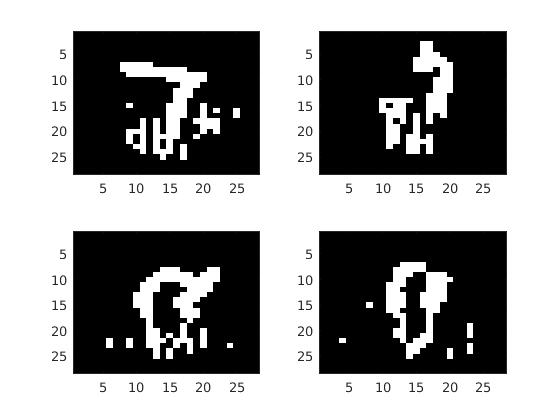
\includegraphics[scale=0.5]{inhomogeneousMC}
\caption{Four samples from an inhomogeneous Markov Chain model}
\end{figure}

\textbf{2 and 3.}
\newline
In this part of the exercise we trained two DAGs where each pixel had $8$ parents and $15$ partents. The parents for the
pixel $(i,j)$ where the pixels in the region $((i-2):i,(j-2):j)$ and $((i-3):i,(j-3):j)$ repectively. The scripts
used to create the model are demoDAG8.m and demoDAG15.m. The results from this different models are shown below.

\begin{figure}[H]
\centering
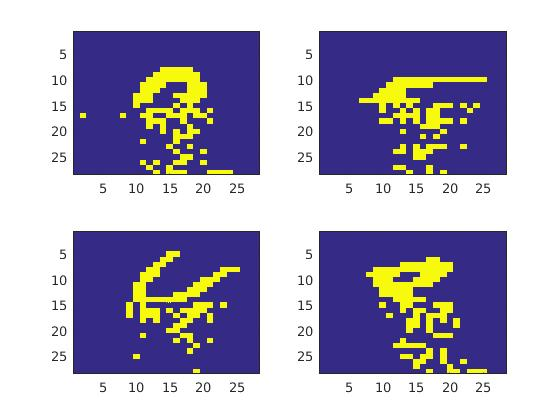
\includegraphics[scale=0.5]{DAG8}
\caption{Four sample images from a DAG model with 8 parents.}
\end{figure}

The results for the DAG with 15 parents are

\begin{figure}[H]
\centering
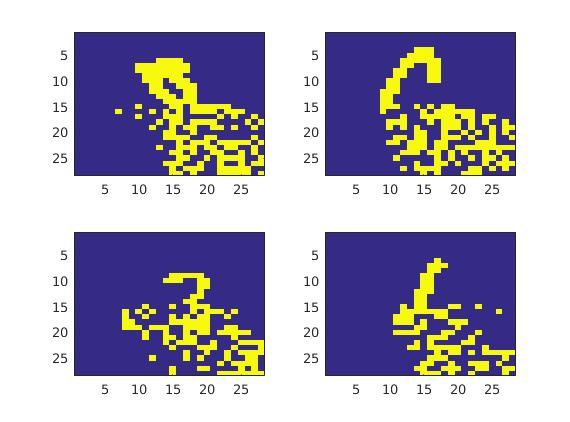
\includegraphics[scale=0.5]{DAG15}
\caption{Four sample images from a DAG model with 15 parents.} 
\end{figure}

It is interesting to see that often the pixel located at $(28,28)$ has value $1$ despite all training images have the value of $0$ at that location.
To understand why this is case consider the parent located at $(25,25)$. There are 16 training images with $1$ in that entry also pixels
$(25,26)$ has five images with that characteristic and $(26,25)$ five images. Hence there are different diffent combinations of vectors
$x_{pa((28,28))}\in\{0,1\}^{15}$ such that
\begin{equation*}
\p(x_{(28,28)=1}|x_{pa((28,28))})\neq 0.
\end{equation*}

\textbf{4.}
Finally we trained a sigmoid belief network where the parents of the pixel located at the point $(i,j)$ are the pixels in the region
$(1:i,1:j)$. we used the script demoSigmoid.m (it takes a couple of minutes to load). The results are shown below.
\end{document}
